\subsection{Resultater}
Fra app'ens hovedmenu kan brugeren tilgå sine resultater. På denne måde er det muligt for brugeren at få et overblik over udviklingen samt udførte træninger.
Aktivitetsdiagrammet over resultater fremgår af \autoref{fig:resultater}.

\begin{figure} [H]
\centering
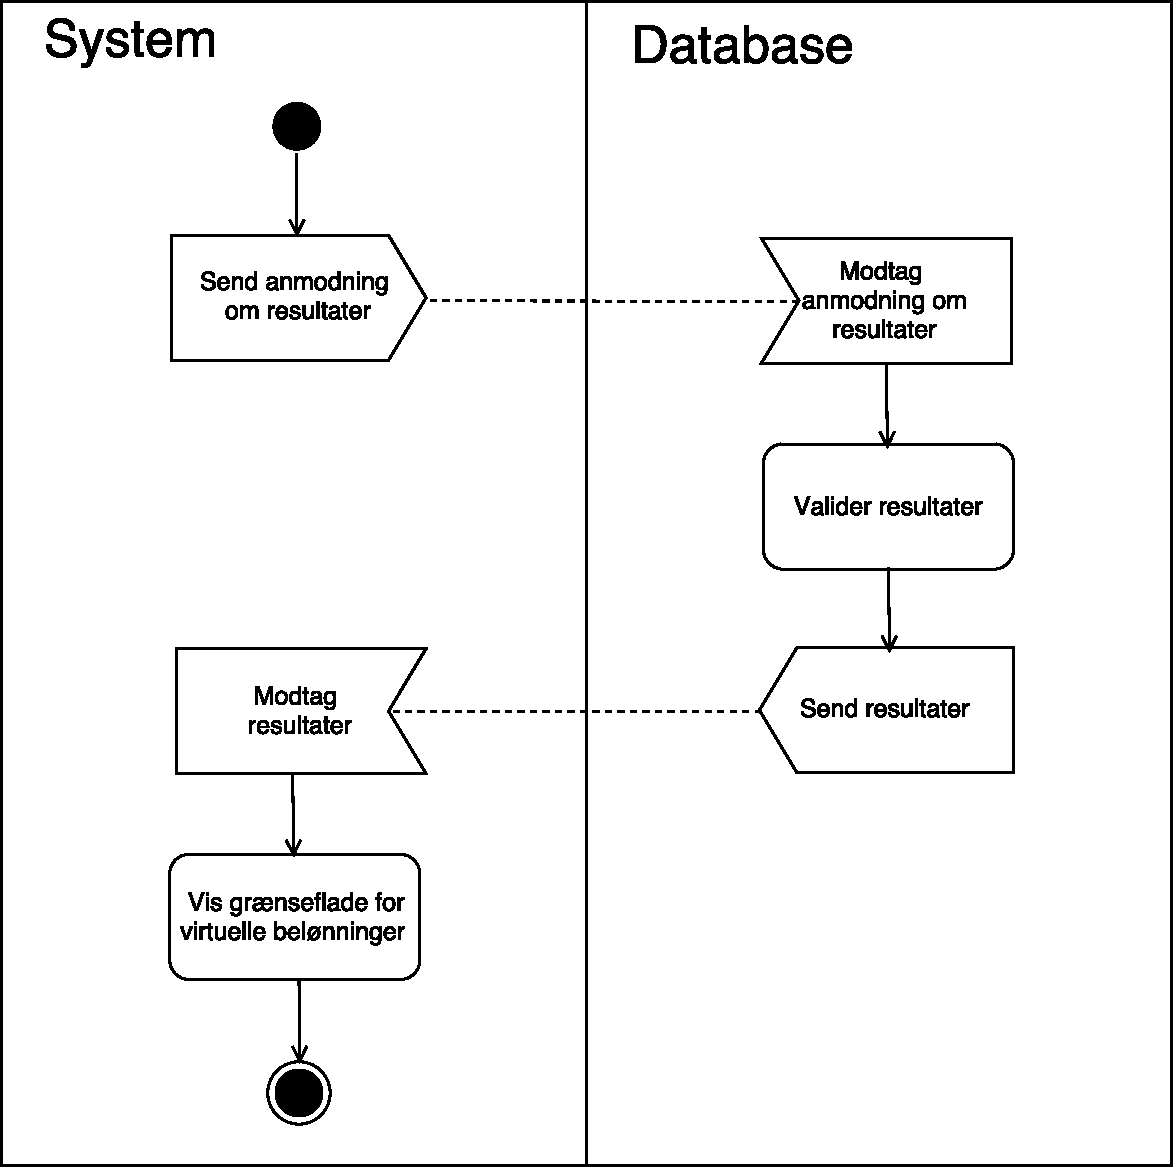
\includegraphics[width=0.9\textwidth]{figures/aktivitetsdiagram/Resultater}
\caption{Aktivitetsdiagram over resultater.}
\label{fig:resultater}
\end{figure}

\noindent
Hvis dette tilgås henter systemet resultater vedrørende brugeren i databasen. Systemet viser grafisk udviklingen af brugerens træning på uge- og månedsbasis. Herefter er der mulighed for at få vist kalender og belønninger. 


I kalenderen kan brugeren få et overblik over, hvilke dage der er udført træning samt de resultater der er opnået de enkelte dage. I belønninger kan brugerne se, hvilke virtuelle belønninger de og andre brugere har opnået i forbindelse med fuldført træning. Belønningerne varierer afhængig af træningsform. Inden for hver træningsform, jf. \autoref{sec:traening}, kan der opnås beløninger inden for forskellige kategorier. Disse kategorier fremgår af \autoref{tab:beloenninger}.

\begin{table} [H]
\centering
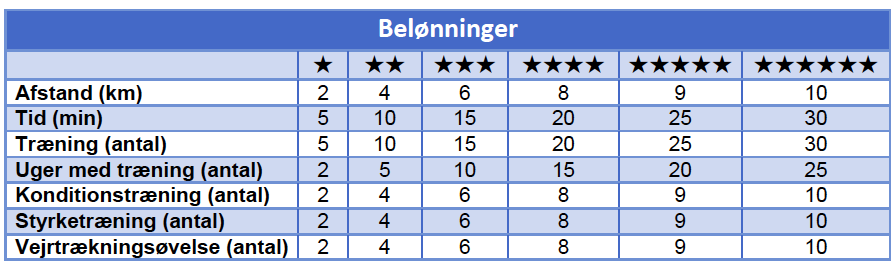
\includegraphics[width=1\textwidth]{figures/aktivitetsdiagram/beloeninnger}
\caption{Belønninger opnået ved træning.}
\label{tab:beloenninger}
\end{table}


\noindent
Ud fra \autoref{tab:beloenninger} fremgår kategorierne der er opdelt efter afstand, tid og gennemførte træninger. Beløningerne opnås forskellige inden for hver kategori og opnås inden for de angivet mål. For eksempel skal man gå 4 km for at opnå XX. 
